\section{Implementierung}
Dies Kapitel dient dazu nachzuvollziehen, wie sich das Programm im Web verhalten würde. Um zu gewährleisten, dass das Programm bei Missverhalten keinen Schaden an dem gerade getesteten Forum anrichtet, wird ein eigenes Forum aufgebaut und ein vollständiger Arbeitszyklus lokal an diesem Forum getestet.

\subsection{Implementierungsumgebung}
Das Forum muss Zugriff auf eine Datenbankquelle haben. Diese besteht für die Dauer der Tests aus Datenbank mit 50.000 Einträgen. Diese Einträge umfassen einen Beitragstitel, einen Beitragsinhalt und eine eindeutige Weburl, die als ID benutzt wird. Die Beiträge sind in einer NoSQL-Datenbank, `Elasticsearch`, gespeichert. Diese bietet den Vorteil, dass mit nur einer Anfrage an die Datenbank in Beitragstitel und Beitragsinhalt, leicht nach einem bestimmten Suchwort gesucht werden kann und die ersten 20 gefundenen Beiträge zurückgeliefert werden.\\
Das Testforum wird lokal erstellt, um eine Vielzahl an Anfragen an ein im Internet verfügbares Forum zu vermeiden. Eine ordentliche Evaluierung könnte einem Internetforum durch zu viel Netzwerkverkehr eventuell schaden.\\
Geschrieben werden alle Programm mit Hilfe von `JavaScript`. Das Forum wird auf einem `Node.js-Server` laufen. 

\subsubsection{Aufbau des Forums}
Das Forum sollte einem originalen Internetforum möglichst nahe kommen, jedoch gleichzeitig eine Umgestaltung der einzelnen Seiten für Anmelden, Registrieren und Suchen nicht allzu aufwändig machen. Dieses erlaubt ein schnelles Debuggen, wenn sich das Programm nicht wie erwartet verhält. Deshalb wird sich beim Erstellen des Forums auf die wichtigsten Elemente konzentriert. Diese umfassen eine Login-, eine Registrierungs- und eine Suchseite.

\subsubsection{Registrierung im Forum}
Die häufigste Registrierungsform, die man in diversen Internetforen findet, besteht aus 2 Feldern für das Passwort, 2 Feldern für die Email, einem Feld für den Nutzernamen und einer Checkbox, in der die Foren-AGB angenommen werden. Dieses wird simpel durch das folgende Codebeispiel demonstriert.

\begin{figure}[h!]
\begin{lstlisting}[language=HTML5]
<form action="/reg" method="post">
Nutzername: <input type="text" name="fname"></br>
Email: <input type="text" name="email"></br>
Validate Email: 
<input type="text" name="re_email"></br>
Password: <input type="password" name="pwd"></br>
Validate Password: 
<input type="password" name="re_pwd"></br>
Accept AGB:<input type="checkbox" name="AGB"></br>
<input type="hidden" name="val1" value="val1">
<input type="hidden" name="val2" value="val2">
<input type="submit" value="Submit">
</form>
\end{lstlisting}
\caption{HTML-Code für die Erstellung einer Registrierungsseite, mit Nutzernamen, Email und Passwordfeldern, sowie Checkbox}
\end{figure}

Aus Abbildung 1 ist es leicht zu evaluieren, ob der Registrierungsprozess erfolgreich sein wird. Zu erwarten wäre ein `POST-Request` an die Toplevel Domain + Formaction mit den POST-Parametern `fname`, `email`, `re\_email`, `pwd`, `re\_pwd`, `AGB`, sowie den hidden Key-Value-Pairs, `val1 = hiddenvalue1` und `val2 = hiddenvalue2`.\\
In die POST-Parameter sollten die entsprechenden Felder, `fname`, `email` und `pwd` jeweils der Name, die Email und das Passwort eingetragen, sowie in den re\_email, re\_pwd jeweils die Email und das Passwort bestätigt sein, indem sie wiederholt eingegeben sind.\\
Ist der HTTP-Server gestartet und wird die Registrierungsseite analysiert und der folgende Request an den Server gesendet :

\begin{figure}[ht]
\begin{lstlisting}[language=HTML5]
/reg
{ val2: 'hiddenvalue2',
val1: 'hiddenvalue1',
AGB: 'on',
re_pwd: 'AjZt198#ev',
pwd: 'AjZt198#ev',
re_email: 'jpm96353@adiaq.com',
email: 'jpm96353@adiaq.com',
fname: 'Dominik' }
verification email to : jpm96353@adiaq.com
\end{lstlisting}
\caption{Inhalt des POST-Requests, den das Programm an das Forum bei einem Registrierungsaufruf sendet}
\end{figure}

Zu beachten ist, dass sich das Programm eine eigene Email angelegt hat. Diese stammt von der Internetseite `10minutemail`\footnote{https://10minutemail.net/ checked: 10.06.2015}.
Diese Internetseite stellt für 10 Minuten eine kostenlose Email-Adresse zur Verfügung, mit der Emails empfangen und gesendet werden können. Die Registrierungsaufforderung wurde an die richtige Url des Servers gesendet, was aus dem `/reg` ersichtlich wird. Weiterhin sind alle erforderlichen Parameter des POST-Requestes und auch die Wiederholungsfelder von Email und Passwort korrekt ausgefüllt worden. Die Checkbox für die AGB wurde angekreuzt und auch alle versteckten Input-Felder der Form mit übertragen. Insgesamt ist dieses eine gültige Registrierungsanfrage, welche der Server mit einer Validierungs-Email an die angegebene Email-Adresse quittiert.

Das Programm überprüft alle 5 Sekunden, ob die Email eingegangen ist. Sollte dieses der Fall sein, wird der Link zur Email aufgerufen, die Email analysiert und jeder darin befindliche Link aufgerufen. Ist innerhalb von 10 Minuten keine Email eingegangen sein, wird der Registrierungsversuch als gescheitert angesehen und dem Nutzer mitgeteilt, denn die Email-Adresse ist nur 10 Minuten valide.

\begin{figure}[ht]
\begin{lstlisting}[language=HTML5]
registered
No new emails
No new emails
No new emails
location='readmail.html?mid=KfKcm0'
https://10minutemail.net/readmail.html?mid=KfKcm0
clicked: http://localhost:12345/validateUser?user=jpm96353@adiaq.com
\end{lstlisting}
\caption{Das Programm wartet auf Registrierungs-Email und ruft alle Links in der Email auf.}
\end{figure}

Der Validierungsversuch wird nun an das Forum gesendet, das den Nutzer als aktiven Nutzer validiert.

\begin{figure}[ht]
\begin{lstlisting}[language=HTML5]
/validateUser?user=jpm96353@adiaq.com
validate:
jpm96353@adiaq.com
\end{lstlisting}
\caption{Forum validiert den Nutzeraccount, da Validierungslink bestätigt wurde.}
\end{figure}

Sollte der Registrierungsprozess nicht funktionieren, kann die Registrierungsform nachgebaut und gegebenfalls Änderungen an den Feldbewertungsmetriken vorgenommen werden um dann erneut auszuprobieren. Danach kann erneut getestet werden ohne Webforen zu belasten. Es gibt auch die Möglichkeit für das Programm, den Registrierungsschritt zu überspringen. Wenn der Nutzer schon einen Nutzeraccount per Hand angelegt hat, kann er das dem Programm über Eingabeparameter mitteilen. Anstatt sich neu zu registrieren, nutzt es nun den vorhandenen Nutzeraccount.

\subsubsection{Forenlogin}
Der Forenlogin sollte bei nicht angegebenen Logindaten mit den zuvor generierten Daten ausgeführt werden. Werden Accountdaten beim Programstart angegeben, sollten diese auch benutzt werden. Der Loginrequest sollte 3 Parameter enthalten, einmal den Nutzernamen und einmal das Passwort. Die Checkbox gibt an, ob man auf der Website eingeloggt bleiben möchte, um bei einem späteren Besuch nicht noch einmal die Nutzerdaten eingeben zu müssen. Das sind die gängigsten Login-Formulare, die im Internet existieren.

\begin{figure}[ht]
\begin{lstlisting}[language=HTML5]
<form action="/log" method="post">
Nutzername: 
<input type="text" name="fname"></br>
Password: 
<input type="password" name="pwd"></br>
Eingeloggt bleiben: 
<input type="checkbox" name="remember">
<input type="submit" value="Submit">
</form>
\end{lstlisting}
\caption{HTML-Code, der die Loginseite des Forums erstellt}
\end{figure}


\begin{figure}[h!]
\begin{lstlisting}[language=HTML5]
loginattempt: 
{fname:'Dominik',
remember: 'on',
pwd:'AjZt198#ev'}
\end{lstlisting}
\caption{Eingehende Loginanfrage des Clients im Forum}
\end{figure}

In Abbildung 6 ist zu sehen, dass alle erforderlichen Daten korrekt ausgefüllt wurden.
\newpage

\begin{figure}[h!]
\begin{lstlisting}[language=HTML5]
loginattempt:
{email: 'jpm96353@adiaq.com',
fname: 'Dominik',
remember: 'on',
pwd: 'AjZt198#ev'}
\end{lstlisting}
\caption{Eingehende Loginanfrage des Clients im Forum mit Nutzername und Email}
\end{figure}
Abbildung 7 zeigt, dass, wenn die Loginform Usernamen und Email abfragen sollte, ein valider Loginrequest abgesendet wird.

\begin{figure}[h!]
\begin{lstlisting}[language=HTML5]
loginattempt:
{email: 'jpm96353@adiaq.com',
fname: 'Dominik',
remember: 'on',
pwd: 'AjZt198#ev',
hiddenvalue: 'v1'}
\end{lstlisting}
\caption{Eingehende Loginanfrage des Clients im Forum mit versteckten Attributen}
\end{figure}

Auch etwaige versteckte Input-Felder werden korrekt gefunden und die Key-Value-Paare in dem POST-Request mit übergeben (Abbildung 8).

Alle nachgebauten Loginseiten diverser im Internet gefundener Seiten wurden im händischen Test erfolgreich ausgefüllt und die zu erwartende Loginanfrage an den Server gesendet.\\
Es ist programmtechnisch möglich sich in Foren automatisch zu registrieren und anzumelden. Im Folgenden müssen nach dem Loginvorgang nun noch relevante Posts zu den jeweiligen Firmenprodukten aus dem Forum extrahiert werden.\\
In Internetforen werden Nutzer, die sich gerade angemeldet haben, auf die Hauptseite des Forums verwiesen. Damit der Browser das realisiert, wird in der Antwort des Servers nach dem erfolgreichen Anmelden ein Statuscode 302 gesendet. Dieser zeigt an, dass der Browser eine andere URL ohne das Zutun des Nutzers laden soll. Die URL steht im Location-Header der Antwort. Dieses muss programmtechnisch realisiert werden, da sonst, ohne den Redirect, bei einer Analyse des HTML Quellcodes keine Suchform gefunden werden könnte, da immer die vorherige, also die Login-Seite analysiert werden würde.\\
Der Server antwortet auf eine erfolgreiche Loginanfrage mit einem Redirect.

\begin{figure}[ht]
\begin{lstlisting}[language=HTML5]
successfull login from: jpm96353@adiaq.com
send 302 to redirect to /main
/main
\end{lstlisting}
\caption{Erfolgreicher Login im Forum und Redirect des Clients zur Hauptseite}
\end{figure}

Der Client überprüft bei jeder Anfrage an den Server, ob der Statuscode sich von 200 (OK) unterscheidet. Sollte es wie in diesem Fall ein 302 (Redirect) sein, wird automatisch die neue URL mit einem GET-Request nachgeladen, damit im nächsten Schritt das neue HTML analysiert werden kann. In diesem Fall wird die Main-Page des Forums als nächstes geladen.

\subsubsection{Suchen im Forum}

\begin{figure}[ht]
\begin{lstlisting}[language=HTML5]
http://localhost:12345/log
{ email: 'jpm96353@adiaq.com',
fname: 'Dominik',
pwd: 'AjZt198#ev',
hiddenvalue: 'v1' }
redirected
redirecturl: /main
\end{lstlisting}
\caption{Client folgt dem Redirect auf die Hauptseite des Forums}
\end{figure}

Der Client erkennt automatisch, dass er auf eine andere Seite verwiesen wurde und lädt diese. Das ist daran zu erkennen, dass das HTML, das im nächsten Schritt analysiert wird, nicht mehr das Login-HTML ist.

\begin{figure}[h!]
\begin{lstlisting}[language=HTML5]
<form accept-charset="UTF-8" action="/search" class="js-site-search-form" data-global-search-url="/search" data-repo-search-url="" method="get">
<div style="margin:0;padding:0;display:inline">
<input name="utf8" type="hidden" value="true"></div>
<input type="text" class="js-site-search-focus chromeless-input" data-hotkey="s" name="q" placeholder="Search OwnForum" data-global-scope-placeholder="Search OwnForum" data-repo-scope-placeholder="Search" tabindex="1" autocapitalize="off">
</form>
\end{lstlisting}
\caption{Zu analysierendes HTML nach dem Redirect enthält die Suchform}
\end{figure}

Dieses HTML wird nach einer Suchform durchsucht. Diese befindet sich meist ein einer GET-Form. Da der Request ein GET-Request ist, wird das Suchwort in der URL codiert. Der Name des Key-Value-Paares, das für die Übermittlung zuständig ist, wird aus den Input-Feldern in der Form generiert. Dieses Attribut hat meist in den Namen `q` oder `search`. Der Client findet diese Suchform und sendet die Suchanfrage an den Server.


\begin{figure}[ht]
\begin{lstlisting}[language=HTML5]
{ action: '/search', name: 'q' }
\end{lstlisting}
\caption{Vom Client analysierte Suchform, gefundener Name des Suchparameters und die Suchurl}
\end{figure}

\newpage


\begin{figure}[ht]
\begin{lstlisting}[language=HTML5]
/search?q=CRM
/search?q=LVM
/search?q=HCM
/search?q=ECOM
\end{lstlisting}
\caption{Eingehende Suchanfragen im Forum }
\end{figure}
Im Forum geht eine valide Suchanfrage ein (Abbildung 13).
Sollte das Suchwort im Titel oder im Beitragsinhalt vorkommen, wird der Link zu diesem Beitrag zurückgegeben. Dieser Link ist in dem Testforum eine eindeutige ID. Es ist anzunehmen, dass die Links in jedem Internetforum eine eindeutige ID für jeden Post darstellen, da sie auf genau eine feste Internetadresse verweisen. So wie in einem Internetforum werden pro Suchwort die ersten 20 Treffer zu diesem Suchwort auf einer HTML zusammengefasst und an den Client ausgeliefert. Zu erwarten ist, dass der Client alle Links speichert und vermerkt, wie oft der Link bei unterschiedlichen Suchworten von dem Forum zurückgegeben wurde. Dazu wird das HTML nach allen vorkommenden Links durchsucht. Des weiteren sollten Links entfernt werden, die in mehr als der Hälfte der Suchanfragen zu finden sind, da es sich hierbei meist um statische Links handelt wie neuste Beiträge oder Links in den Navigationsleisten.
\newpage

\begin{figure}[h!]
\begin{lstlisting}[language=JavaScript]
dispatcher.onGet("/search", function(req, res) {
res.writeHead(200, {'Content-Type': 'text/html'})
var results = searchDataBaseForWord(req.params.q)
.then(function(results){
if(results.length > 0){
var temp = ''
for (var i = results.length - 1; i >= 0; i--) {
temp += '<a href="/'+ results[i] +'">Link</a>'
temp += '</br>'
}
temp +='<a href="/shouldberemovedLink">REMOVELINK</a>'
temp += '</br>'
res.write(temp)
}else{
var temp = ''
temp +='<a href="/shouldberemovedLink">REMOVELINK</a>'
temp += '</br>'
temp += "<h1> No valid Data found </h1>"
res.write(temp)
}
res.end() 
}) 
})
\end{lstlisting}
\caption{Erstellung der Ergebnisseite auf eine Suchanfrage im Forum}
\end{figure}

In Abbildung 14 wird für jede Suchanfrage das HTML erstellt, das die Links zu den jeweiligen passenden Dokumenten enthält. Diese Links stammen aus der Datenbankabfrage mit dem entsprechenden Suchwort.
Ein statischer Link, der wiederum die statischen Links, auf Internetseiten simulieren soll, wird platziert. Er sollte danach vom Client wieder entfernt werden, da in mehr als der Hälfte der Anfragen vorhanden ist und somit wahrscheinlich keinen Link zu einem Beitrag darstellt.

\begin{figure}[h!]
\begin{lstlisting}[language=HTML5]
/search?q=besiege
/search?q=briar
/search?q=individuals
/search?q=evacuate
/search?q=steals
/search?q=detrimental
/search?q=untimely
/search?q=bestir
/search?q=graphical
/search?q=revelation
\end{lstlisting}
\caption{10 Suchanfragen des Clients an das Forum, mit zufälligen Wörtern}
\end{figure}

\begin{figure}[h!]
\begin{lstlisting}[language=HTML5]
{"href=\"/g-1814892-S-5993338243263848452\"":1,
"href=\"/g-1850237-S-6005730948694503428\"":1,
"href=\"/g-115178-S-5999229826848821253\"":1,
"href=\"/g-66325-S-6001320511865446402\"":1,
"href=\"/g-66325-S-6003599070168440836\"":1,
"href=\"/g-54723-S-5999922118567956482\"":1}
\end{lstlisting}
\caption{Gesammelte Dokumente des Clients auf die 10 Suchanfragen}
\end{figure}

Bei 10 Suchanfragen an die Datenbank (Abbildung 15) mit zufälligen englischen Wörtern wurden 6 Dokumente in der Testdatenbank gefunden (Abbildung 16). Keines wurde doppelt getroffen und der statische Link wurde entfernt. Die verbleibenden Links können nun mit einem GET-Request an den entsprechenden Link heruntergeladen und indexiert werden.
\newpage

\begin{figure}[h!]
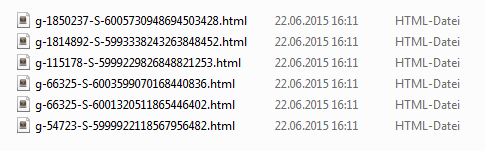
\includegraphics{./images/postdownload.png}
\caption{Heruntergeladne HTML-Seiten der Beiträge der Suchanfragen}
\end{figure}


Es wurden erfolgreich die 6 Dokumente des Forums heruntergeladen, die das Forum auf die 10 Suchanfragen ausgeliefert hat.
Damit ist gezeigt, das es möglich ist, sich automatisch in Foren zu registrieren , einzuloggen und nach bestimmten (firmenspezifischen) Schlagworten für Produkte zu suchen.

